\noindent
\begin{minipage}[t]{0.26\textwidth}
    % Cột lề: ghi chú bên lề và các hình vẽ dóng hàng theo tọa độ gốc
    \vspace*{142pt} % Dóng hàng chuẩn xác với định nghĩa của Ví dụ 7
    \noindent
    {\small Kết quả của Ví dụ 7 có vẻ hợp lý khi quan sát Hình 3.\par}
    
    \vspace{6pt}
    \centering
    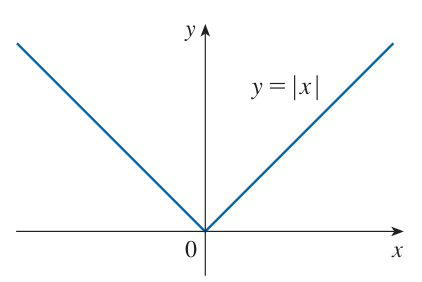
\includegraphics[width=0.98\linewidth]{images/p0135_fig1.png}
    
    \vspace{3pt}
    \raggedright
    {\small\textbf{\textsf{HÌNH 3}}\par}
    
    \vspace{38pt} % Dóng hàng chuẩn xác với các phép tính giới hạn của Ví dụ 8
    \centering
    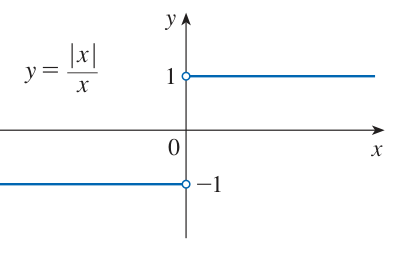
\includegraphics[width=0.98\linewidth]{images/p0135_fig2.png}
    
    \vspace{3pt}
    \raggedright
    {\small\textbf{\textsf{HÌNH 4}}\par}
\end{minipage}%
\hfill
\begin{minipage}[t]{0.71\textwidth}
    % Cột chính: Lý thuyết, Định lý và các Ví dụ
    \vspace{0pt}
    \noindent
    {\color{stewartcyan}\rule{6.5pt}{6.5pt}}\hspace{0.5em}\textbf{\textsf{\large Sử dụng các giới hạn một phía}}

    \vspace{2pt}
    Một số giới hạn được tính toán tốt nhất bằng cách trước tiên tìm các giới hạn bên trái và bên phải. Định lý sau đây nhắc lại những gì chúng ta đã khám phá trong Mục 2.2. Định lý khẳng định rằng giới hạn hai phía tồn tại khi và chỉ khi cả hai giới hạn một phía đều tồn tại và bằng nhau.

    \vspace{2pt}
    \begin{tcolorbox}[
        colframe=stewartred,
        colback=white,
        boxrule=0.7pt,
        arc=0pt,
        left=8pt,
        right=8pt,
        top=6pt,
        bottom=6pt
    ]
        \noindent
        {\color{stewartred}\fbox{\textbf{\small 1}}}\hspace{0.5em}%
        \textbf{\textsf{\color{stewartred}Định lý}}\hspace{1.5em}%
        $\displaystyle\lim_{x \to a} f(x) = L \quad\text{khi và chỉ khi}\quad \lim_{x \to a^-} f(x) = L = \lim_{x \to a^+} f(x)$
    \end{tcolorbox}

    \vspace{2pt}
    Khi tính toán các giới hạn một phía, chúng ta sử dụng sự kiện rằng các Quy tắc giới hạn cũng đúng cho các giới hạn một phía.

    \vspace{4pt}
    \noindent
    \textbf{\textsf{\color{stewartcyan}VÍ DỤ 7}}\hspace{1em}Chứng minh rằng $\displaystyle\lim_{x \to 0} |x| = 0$.

    \vspace{2pt}
    \noindent
    \textbf{\textsf{\color{stewartcyan}LỜI GIẢI}}\hspace{1em}Nhắc lại rằng
    \[
    |x| = \begin{cases} 
    x & \text{nếu } x \ge 0 \\ 
    -x & \text{nếu } x < 0 
    \end{cases}
    \]
    Vì $|x| = x$ với $x > 0$, ta có
    \[
    \lim_{x \to 0^+} |x| = \lim_{x \to 0^+} x = 0
    \]
    Với $x < 0$, ta có $|x| = -x$ và do đó
    \[
    \lim_{x \to 0^-} |x| = \lim_{x \to 0^-} (-x) = 0
    \]
    Do đó, theo Định lý 1,
    \[
    \lim_{x \to 0} |x| = 0 \tag*{\color{stewartcyan}\blacksquare}
    \]

    \vspace{3pt}
    \noindent
    \textbf{\textsf{\color{stewartcyan}VÍ DỤ 8}}\hspace{1em}Chứng minh rằng $\displaystyle\lim_{x \to 0} \frac{|x|}{x}$ không tồn tại.

    \vspace{2pt}
    \noindent
    \textbf{\textsf{\color{stewartcyan}LỜI GIẢI}}\hspace{1em}Sử dụng các sự kiện rằng $|x| = x$ khi $x > 0$ và $|x| = -x$ khi $x < 0$, ta có
    \[
    \lim_{x \to 0^+} \frac{|x|}{x} = \lim_{x \to 0^+} \frac{x}{x} = \lim_{x \to 0^+} 1 = 1
    \]
    \[
    \lim_{x \to 0^-} \frac{|x|}{x} = \lim_{x \to 0^-} \frac{-x}{x} = \lim_{x \to 0^-} (-1) = -1
    \]
    Vì giới hạn bên phải và giới hạn bên trái khác nhau, theo Định lý 1 suy ra rằng $\lim_{x \to 0} |x|/x$ không tồn tại. Đồ thị của hàm số $f(x) = |x|/x$ được thể hiện trong Hình 4 và hoàn toàn phù hợp với các giới hạn một phía mà chúng ta đã tìm được.\hfill{\color{stewartcyan}\rule{1.2ex}{1.2ex}}

    \vspace{5pt}
    \noindent
    \textbf{\textsf{\color{stewartcyan}VÍ DỤ 9}}\hspace{1em}Nếu
    \[
    f(x) = \begin{cases} 
    \sqrt{x - 4} & \text{nếu } x > 4 \\ 
    8 - 2x & \text{nếu } x < 4 
    \end{cases}
    \]
    hãy xác định xem $\displaystyle\lim_{x \to 4} f(x)$ có tồn tại hay không.
\end{minipage}

\vfill
\noindent
\begin{minipage}{\textwidth}
    \centering
    \fontsize{6.5}{8}\selectfont\color{gray!80}
    Copyright 2021 Cengage Learning. All Rights Reserved. May not be copied, scanned, or duplicated, in whole or in part. WCN 02-200-203
\end{minipage}
